\section{EVALUATION}
\uline{\textbf{Simulations}}: Our algorithm was implemented in MATLAB. Three case studies of path planning are considered for validation: same location and different orientation between initial configuration and goal configuration, long distance between two configuration, and bi-direction path finding.\\

\noindent\uline{\textbf{Cube solid}}:
Writing about cube solid properties\\

\noindent\uline{Case study 1}: Dennis also went his own way and divided the sides of the triangles into equal-angles (as measured from the center of the geodesic), instead of equal-length pieces. This technique is slightly more effective at evenly distributing the triangles across the surface of the sphere. For example, compare an octahedron subdivided with frequency 20, using the linear technique (as outlined by the quiz) versus the angular technique Dennis used in this picture. Note how the linear technique has the triangles piling up along the edges of the original face of the octahedron, where the radial technique does a better job of spacing them out.
\begin{center}
\begin{figure}[h]
\subfigure[The initial configuration is the same position but different orientation with goal configuration]{
	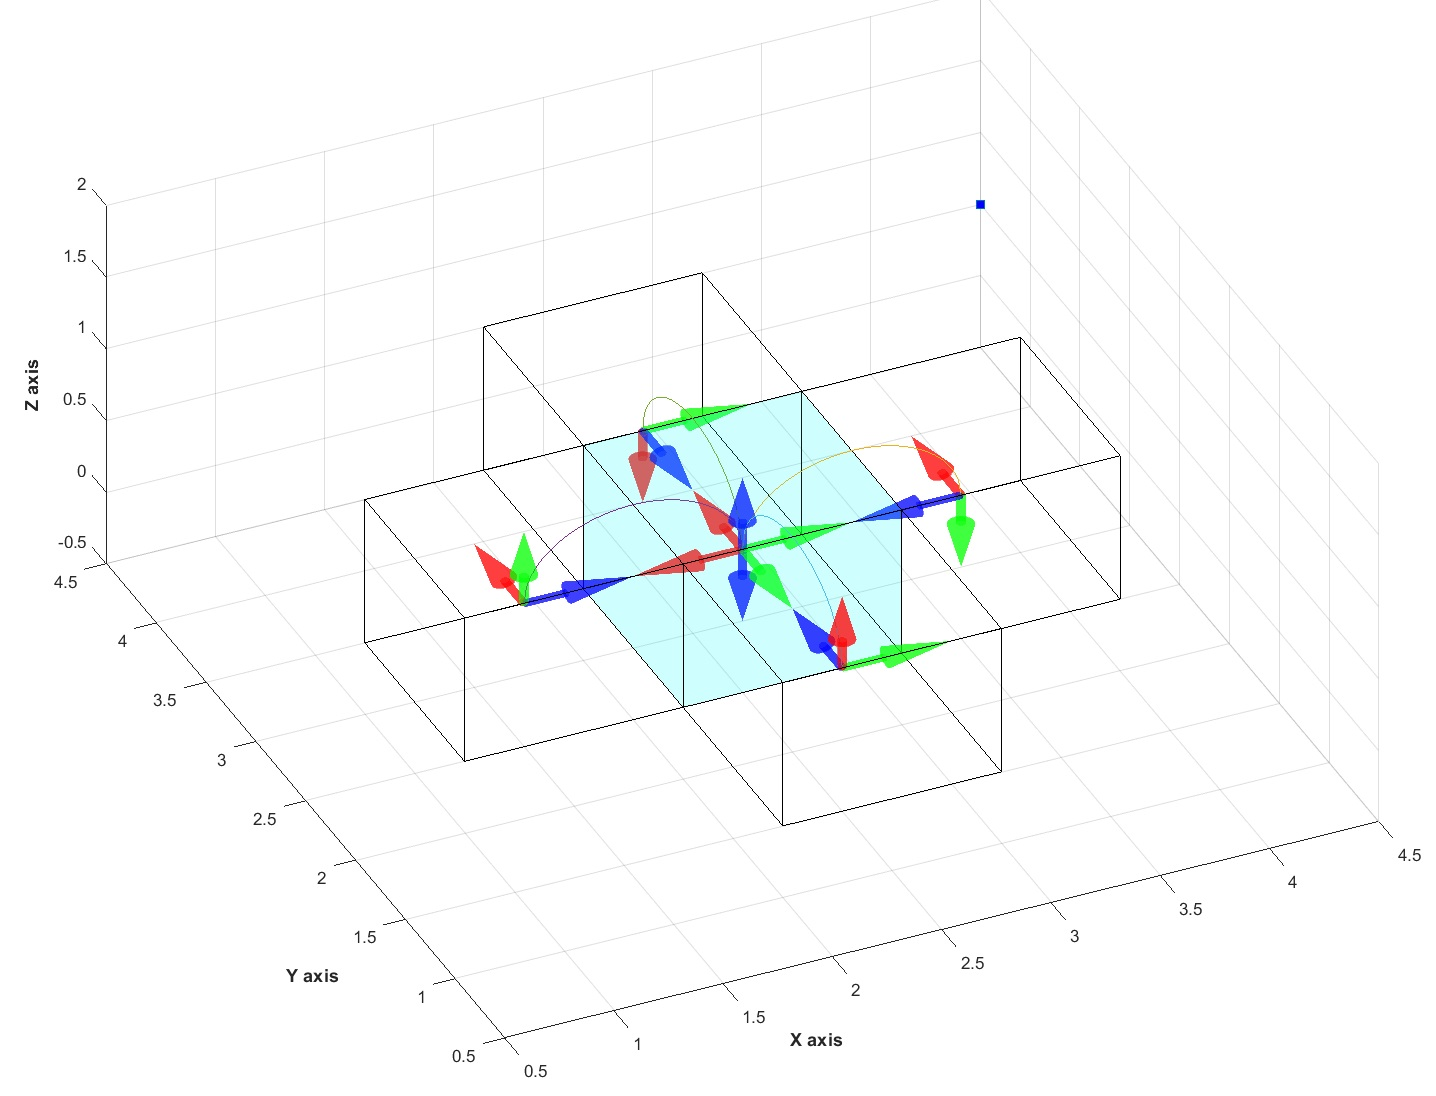
\includegraphics[width=0.5\textwidth]{image/cube11.jpg}
	\label{fig:Cube1Case1}
	}
\hfill
\subfigure[First four paths of the cube rolling]{
	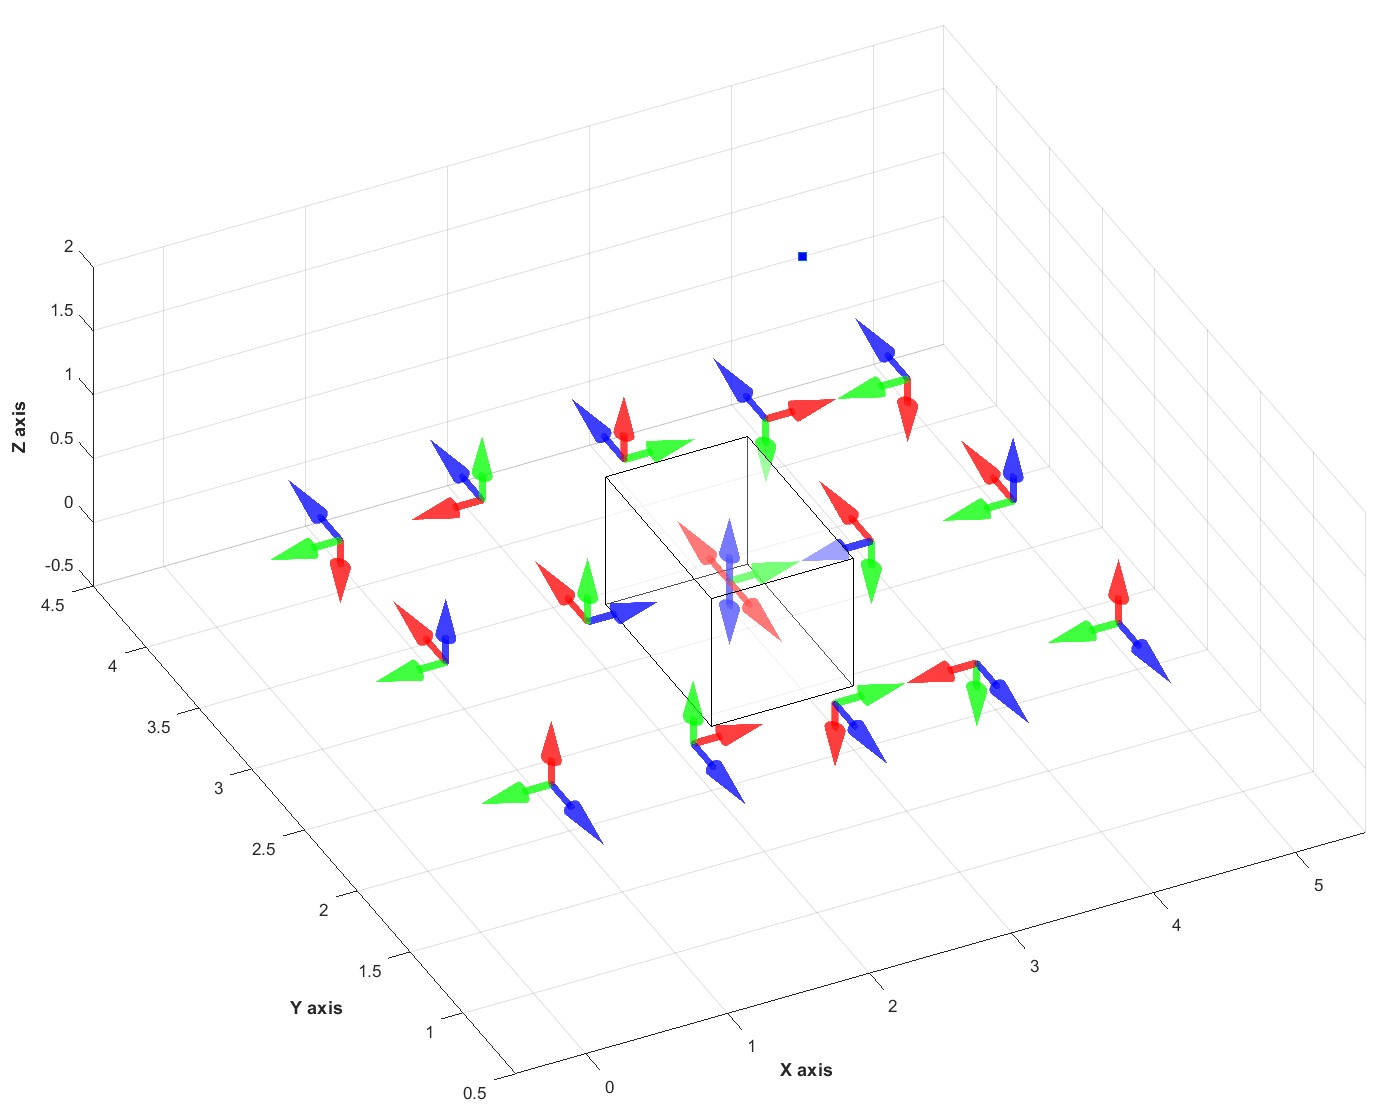
\includegraphics[width=0.5\textwidth]{image/cubePath4Dirs.jpg}
%    \includegraphics[page=2,width=.5\textwidth]{image/test2.pdf}	
	\label{fig:Cube2Case1}
	}
\caption{Blah Blah}
\end{figure}
\end{center}

\noindent\uline{Result}: 
\begin{figure}[h]
\centering
	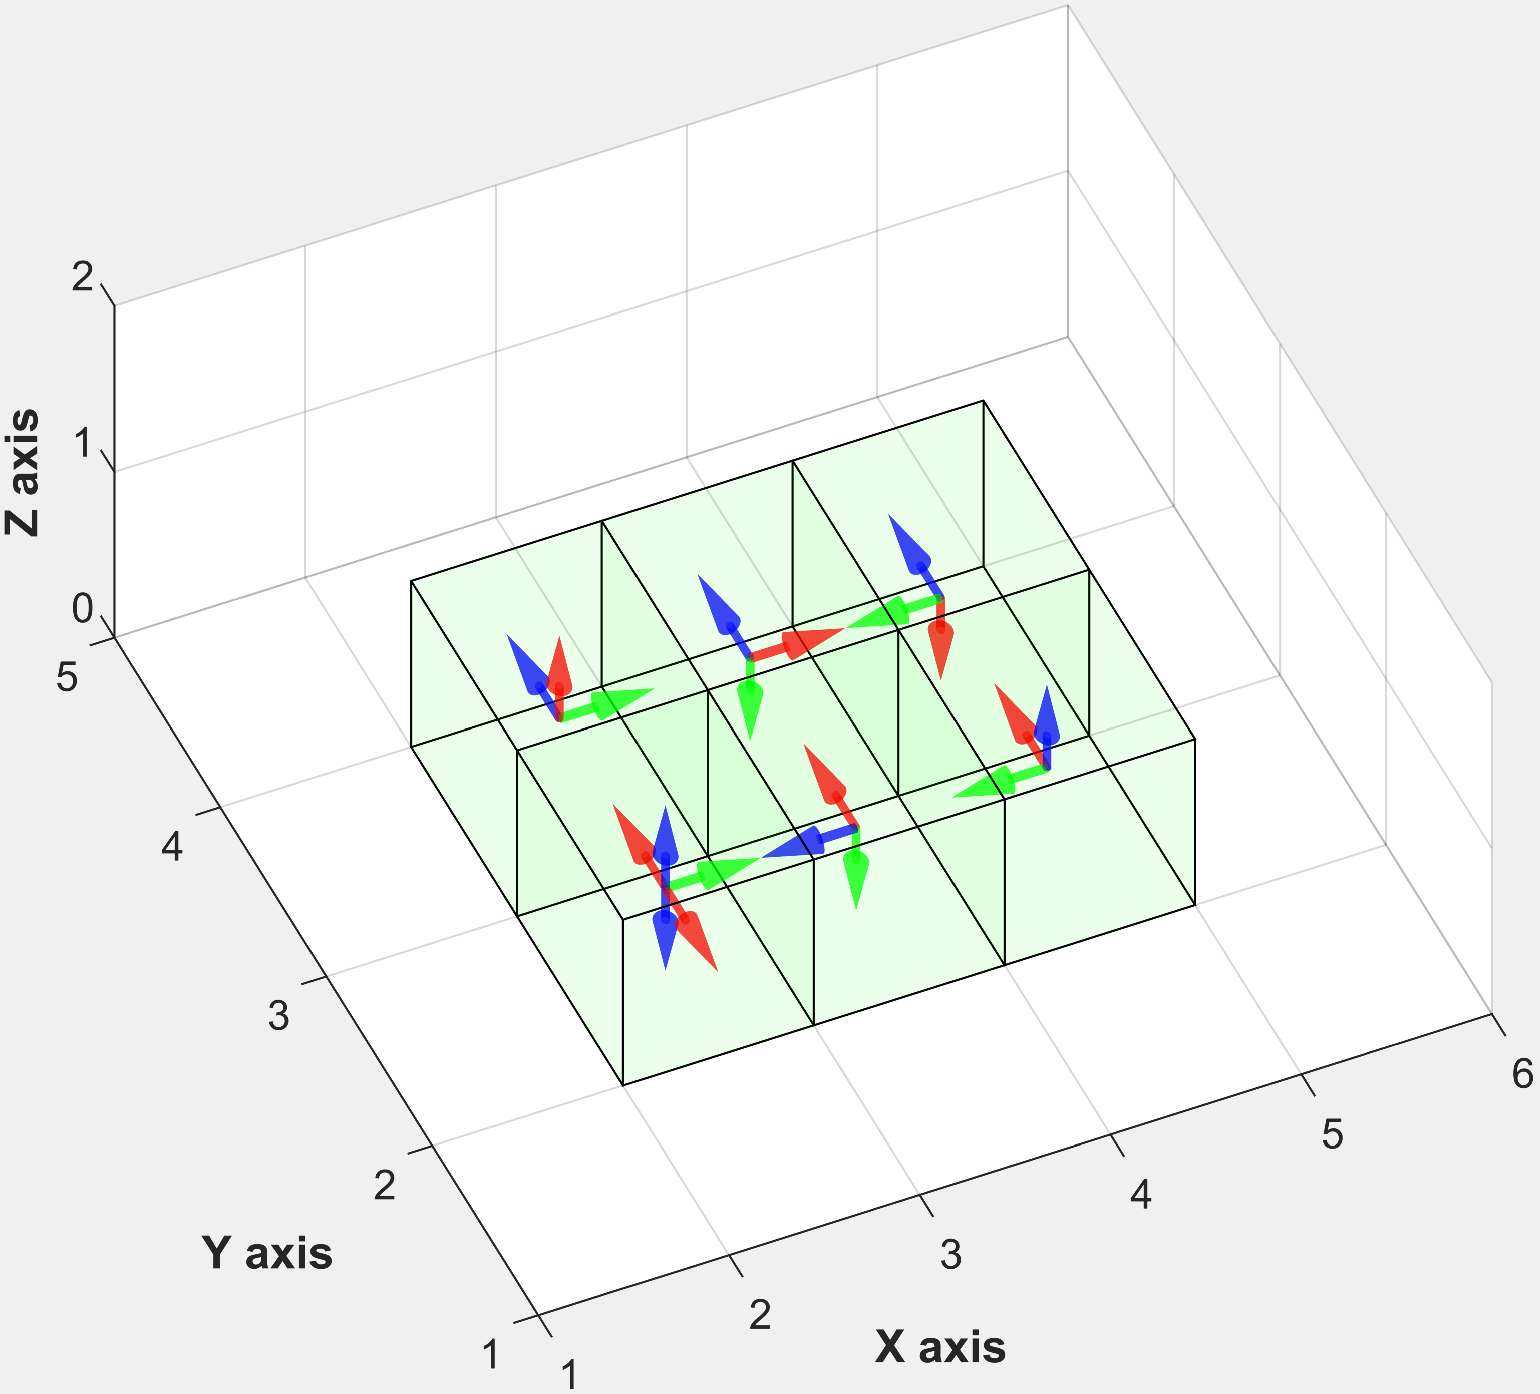
\includegraphics[width=1\textwidth]{image/cubePath1.pdf}
	\caption{Shortest path of cube rolling}
	\label{fig:cubePath1}
\end{figure}

%\begin{figure}[h]
%	\centering
%		\begin{subfigure}[t]
%			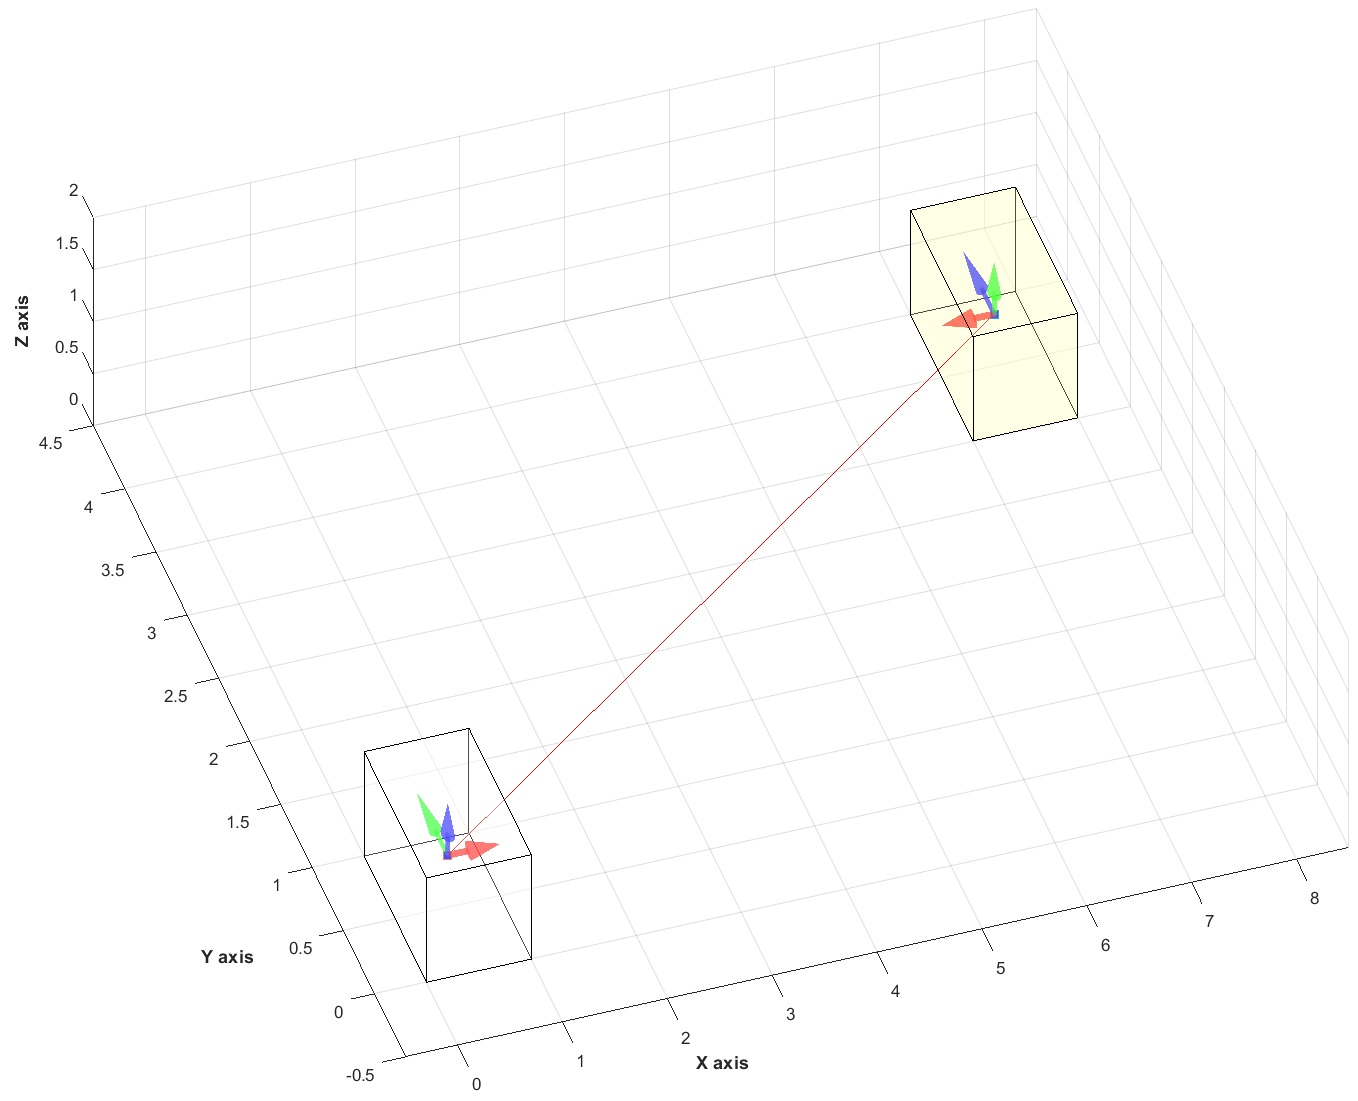
\includegraphics[width=0.5\textwidth]{image/cubePathCase2Initial.jpg}
%			\subcaption{Long distance between two configurations}
%			\label{fig:Cube1Case2}
%		\end{subfigure}
%%\hfill
%		\begin{subfigure}[t]
%			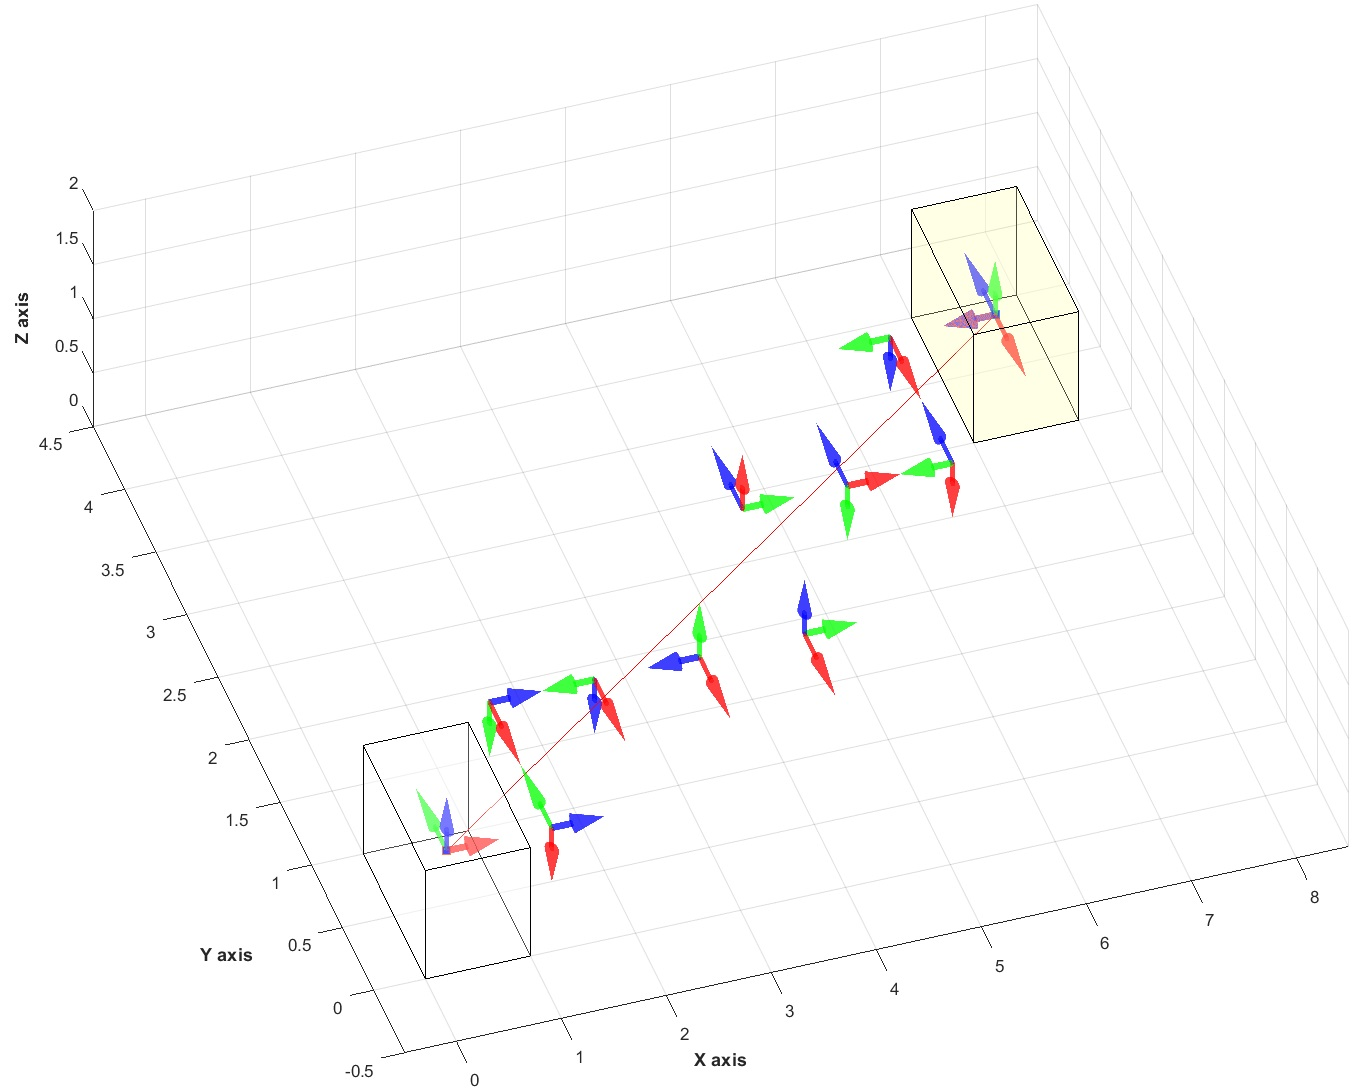
\includegraphics[width=0.5\textwidth]{image/cubePathCase2DirecRolling.jpg}
%			\subcaption{Directly rolling from initial configuration to goal configuration}
%			\label{fig:Cube2Case2}
%		\end{subfigure}
%\end{figure}

%%
%%
%%
\begin{center}
\begin{figure}[h]
\subfigure[Path1]{
	\includegraphics[width=0.5\textwidth]{image/cubeCase2Path1.jpg}
	\label{fig:Cube3Case2}
	}
\hfill
\subfigure[Path2]{
	\includegraphics[width=0.5\textwidth]{image/cubeCase2Path2.jpg}
	\label{fig:Cube4Case2}
	}
\caption{Blah Blah 3}
\end{figure}
\end{center}
%%
%%
%%
%%
%%==================================================================================
%%
%%==================================================================================
%%
%%
%%
\clearpage
\newpage
\noindent\uline{\textbf{Tetrahedron solid}}:
Writing about cube solid properties\\

\noindent\uline{Case study 1}:
Dennis also went his own way and divided the sides of the triangles into equal-angles (as measured from the center of the geodesic), instead of equal-length pieces. This technique is slightly more effective at evenly distributing the triangles across the surface of the sphere. For example, compare an octahedron subdivided with frequency 20, using the linear technique (as outlined by the quiz) versus the angular technique Dennis used in this picture. Note how the linear technique has the triangles piling up along the edges of the original face of the octahedron, where the radial technique does a better job of spacing them out.\\

\begin{center}
\begin{figure}[h]
\subfigure[The initial configuration is the same position but different orientation with goal configuration]{
	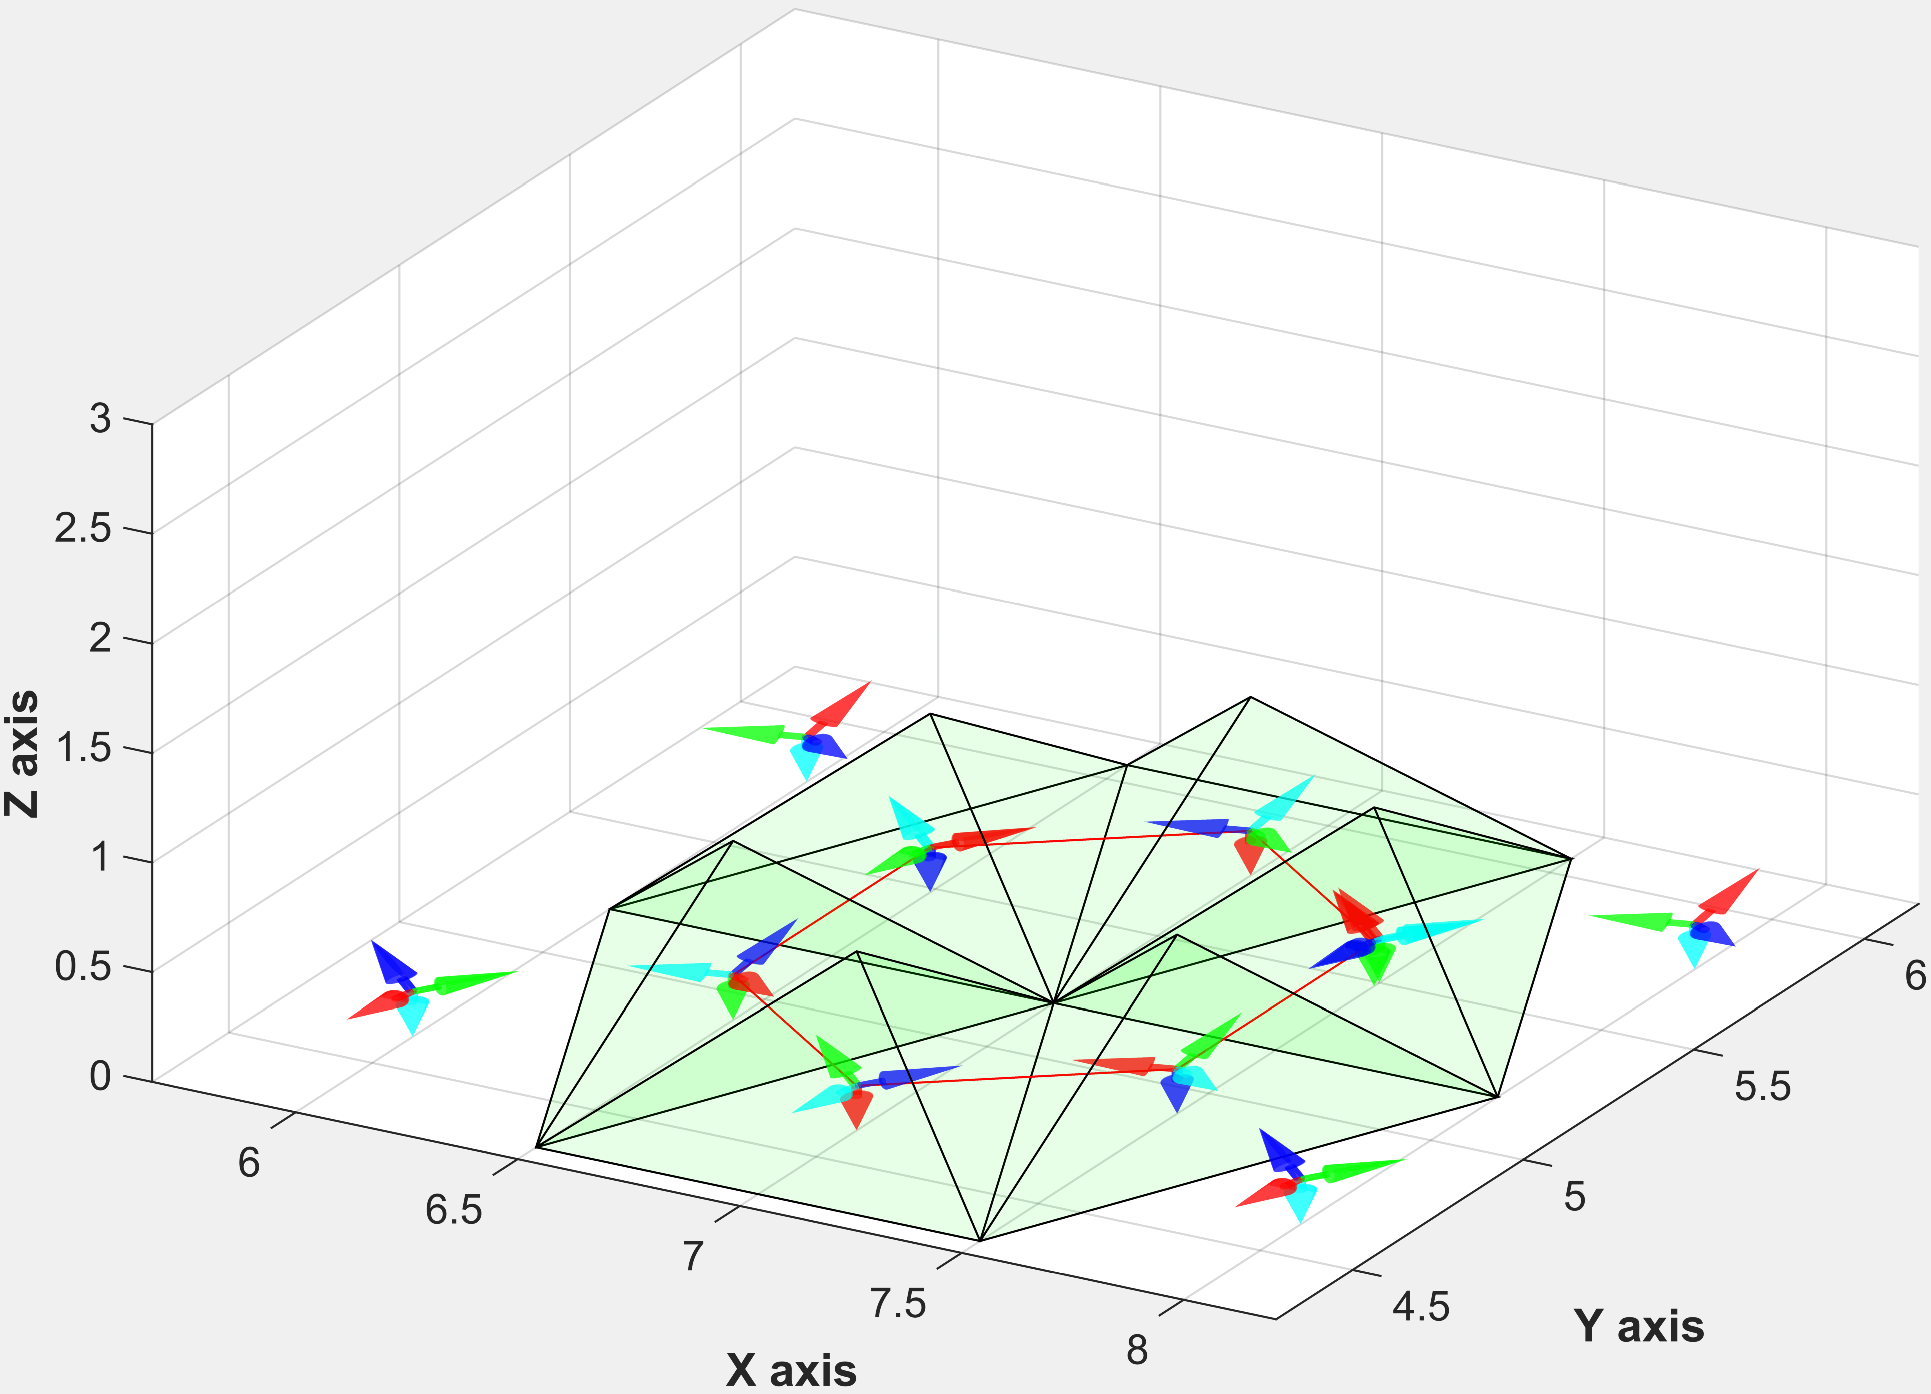
\includegraphics[width=0.5\textwidth]{image/tetraPath2.pdf}
	\label{fig:Tetra1Case1}
	}
\hfill
\subfigure[First four paths of the cube rolling]{
	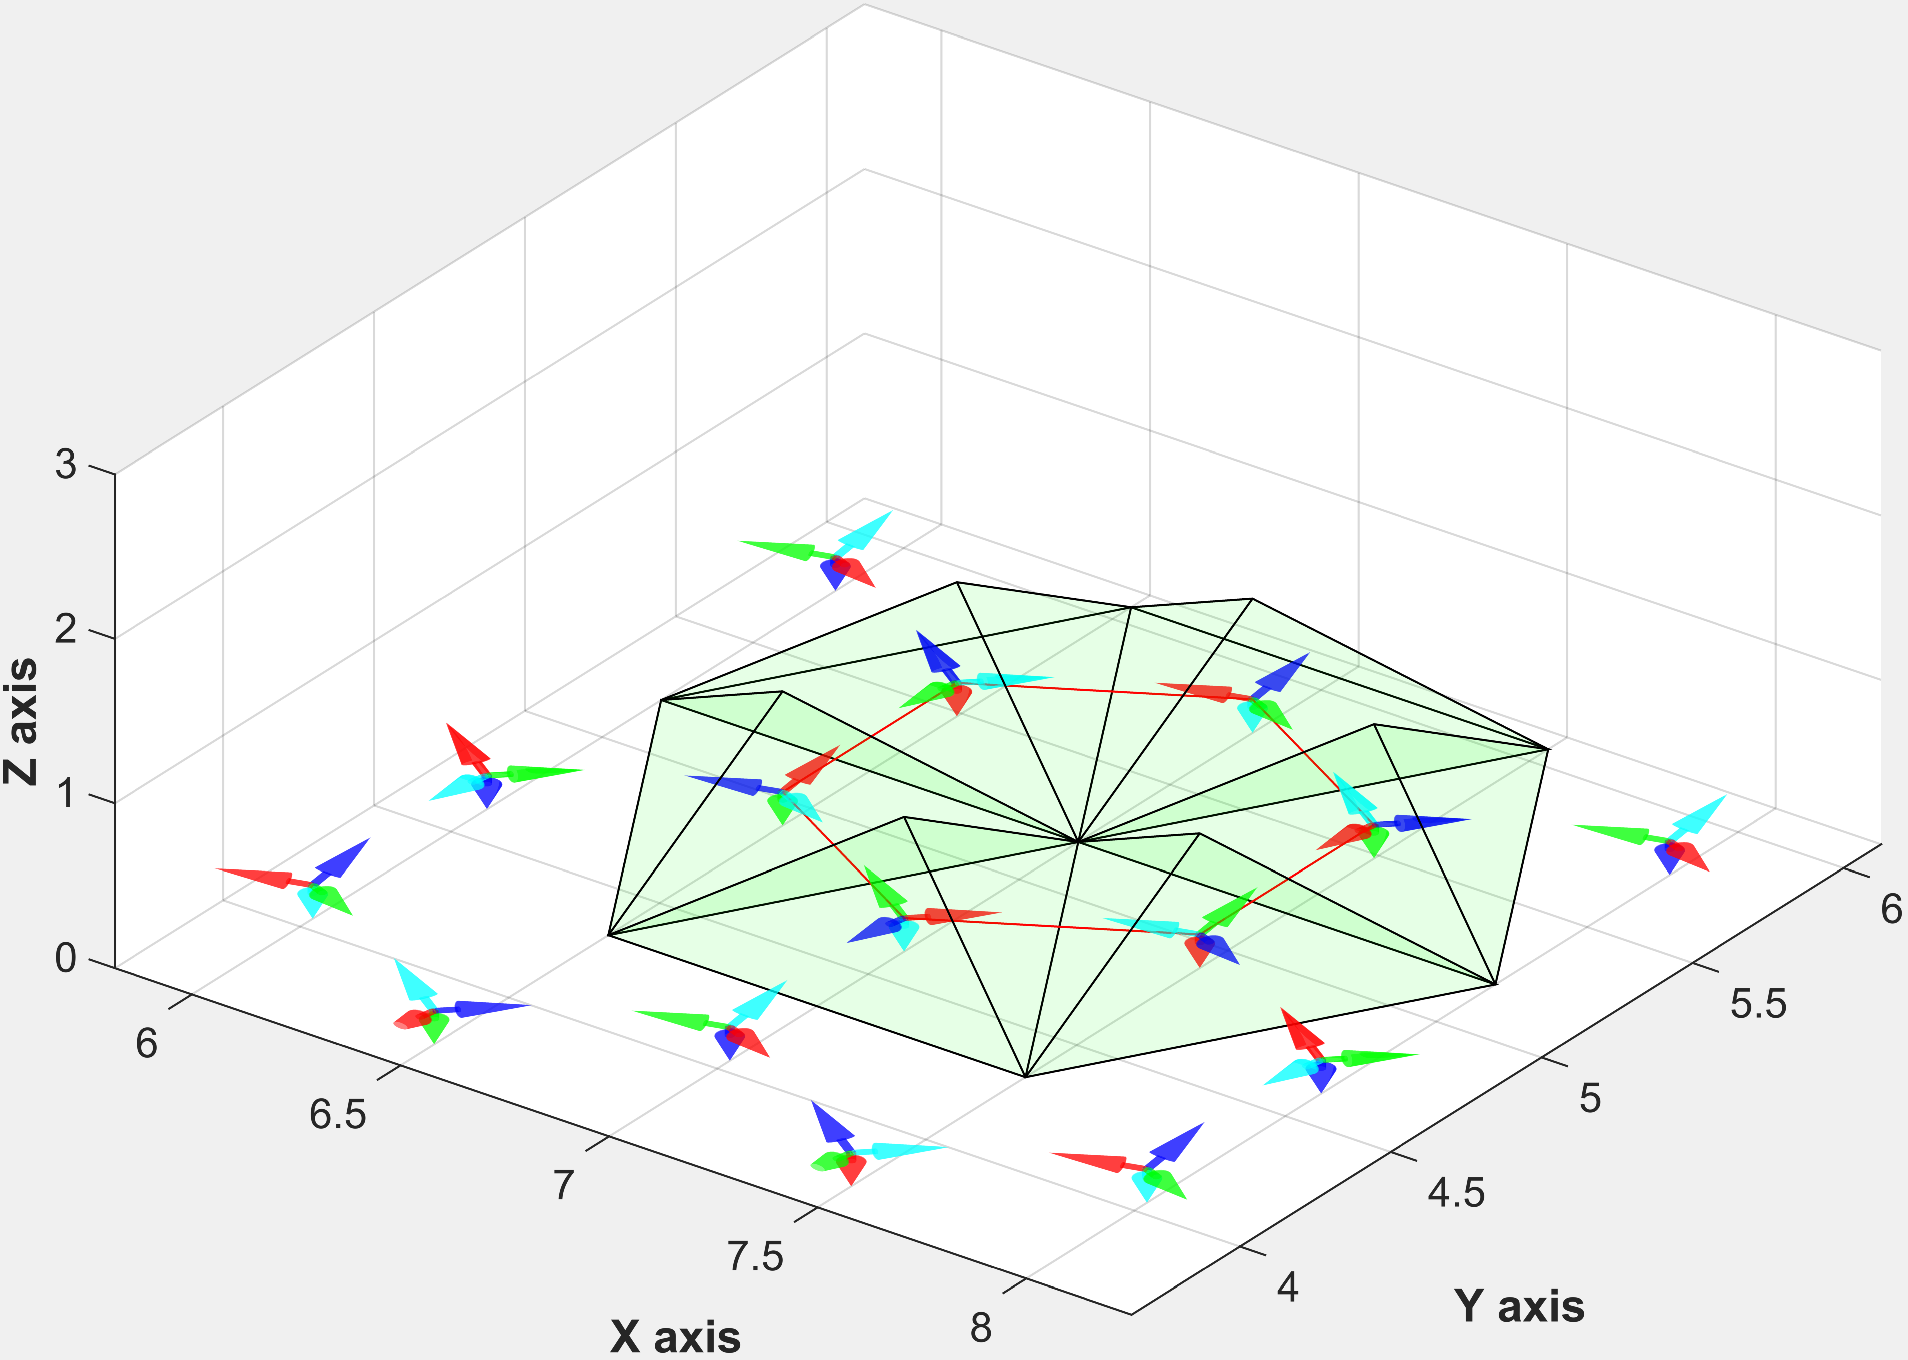
\includegraphics[width=0.5\textwidth]{image/tetraPath1.pdf}
	\label{fig:Tetra2Case1}
	}
\caption{Blah Blah Tetra}
\end{figure}
\end{center}
%%
%%
%%
%%==================================================================================
%%
%%==================================================================================
%%
%%
%%
\clearpage
\newpage
\noindent\uline{\textbf{Octahedron solid}}:
Dennis also went his own way and divided the sides of the triangles into equal-angles (as measured from the center of the geodesic), instead of equal-length pieces. This technique is slightly more effective at evenly distributing the triangles across the surface of the sphere. For example, compare an octahedron subdivided with frequency 20, using the linear technique (as outlined by the quiz) versus the angular technique Dennis used in this picture. Note how the linear technique has the triangles piling up along the edges of the original face of the octahedron, where the radial technique does a better job of spacing them out.\\

\begin{center}
\begin{figure}[h]
\subfigure[The first shortest path of Octahedron path rolling]{
	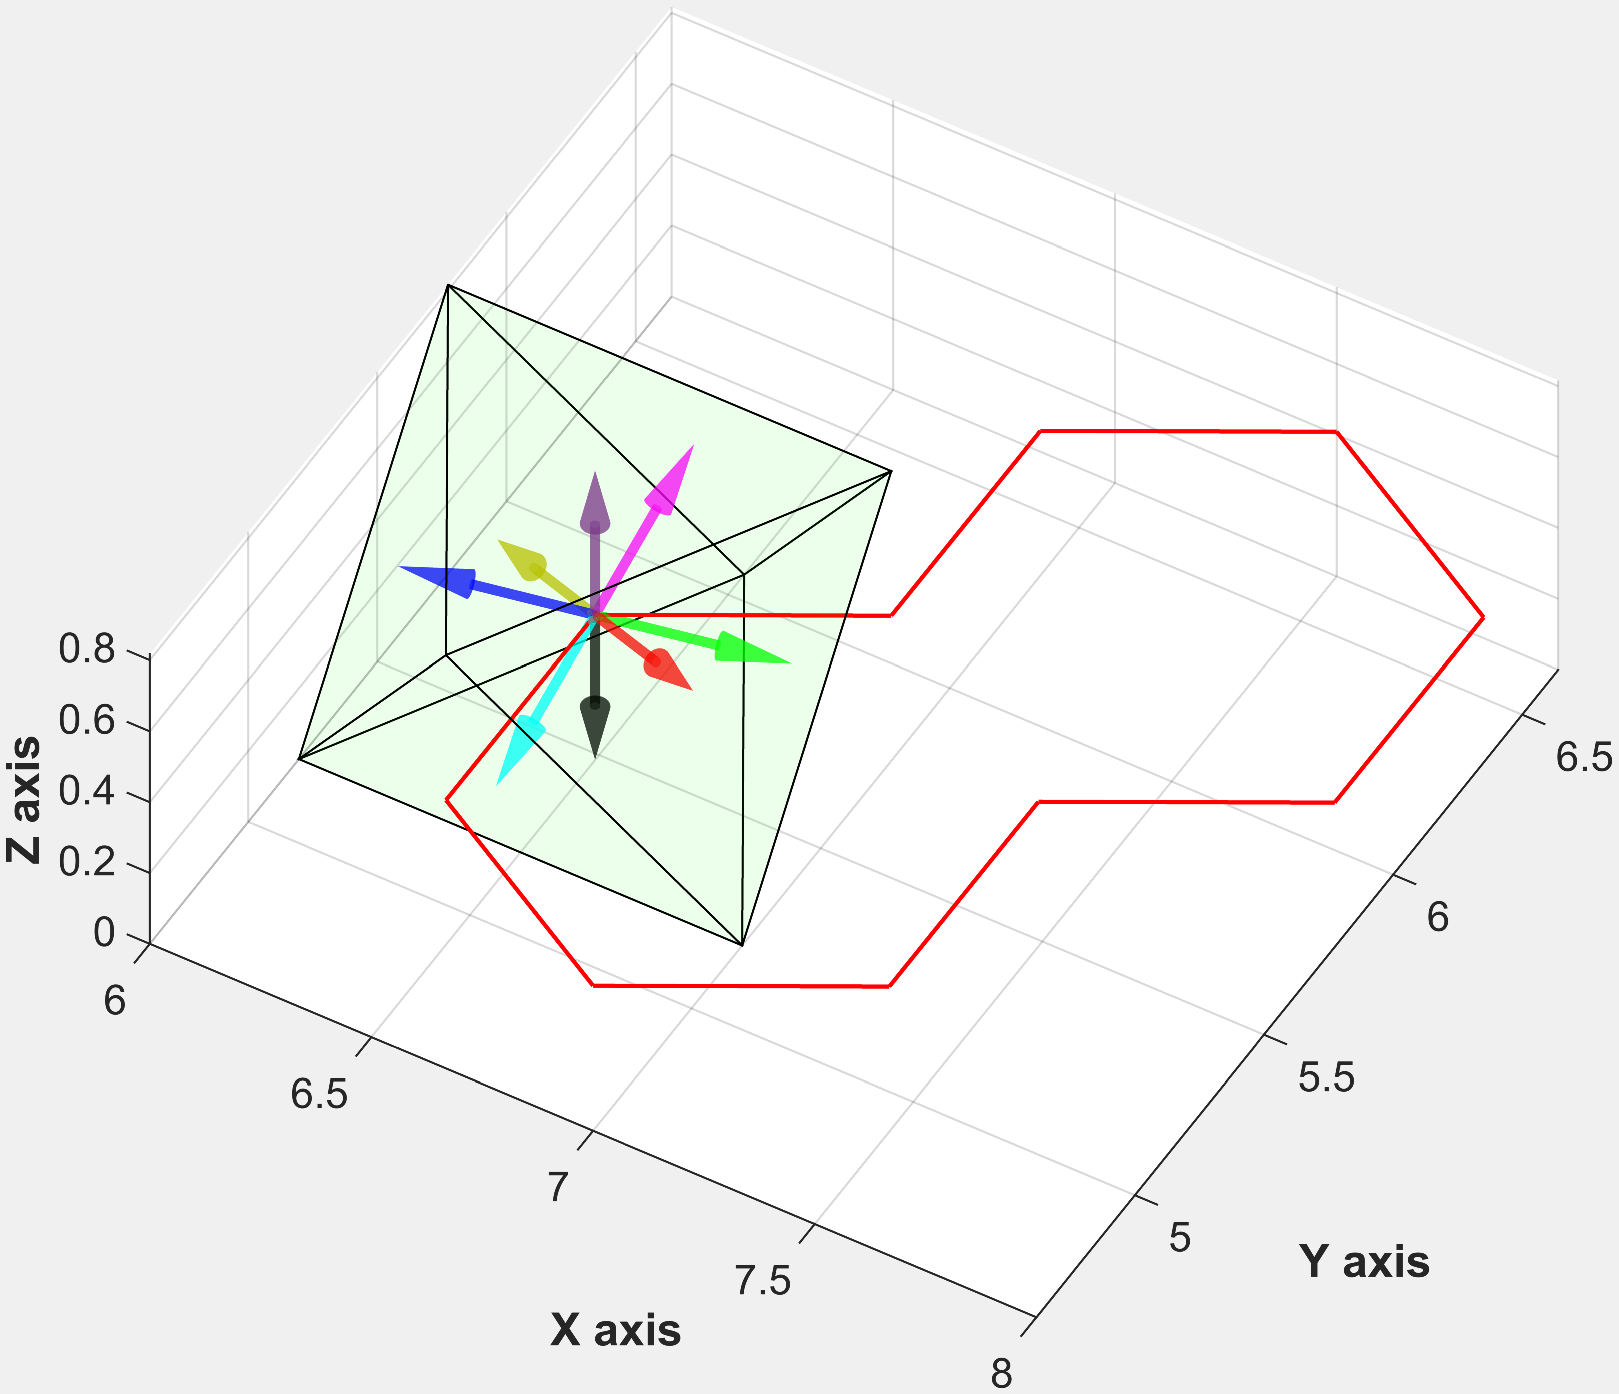
\includegraphics[width=0.5\textwidth]{image/octoPath1.pdf}
	\label{fig:Octa1Case1}
	}
\hfill
\subfigure[The second shortest path of Octahedron path rolling]{
	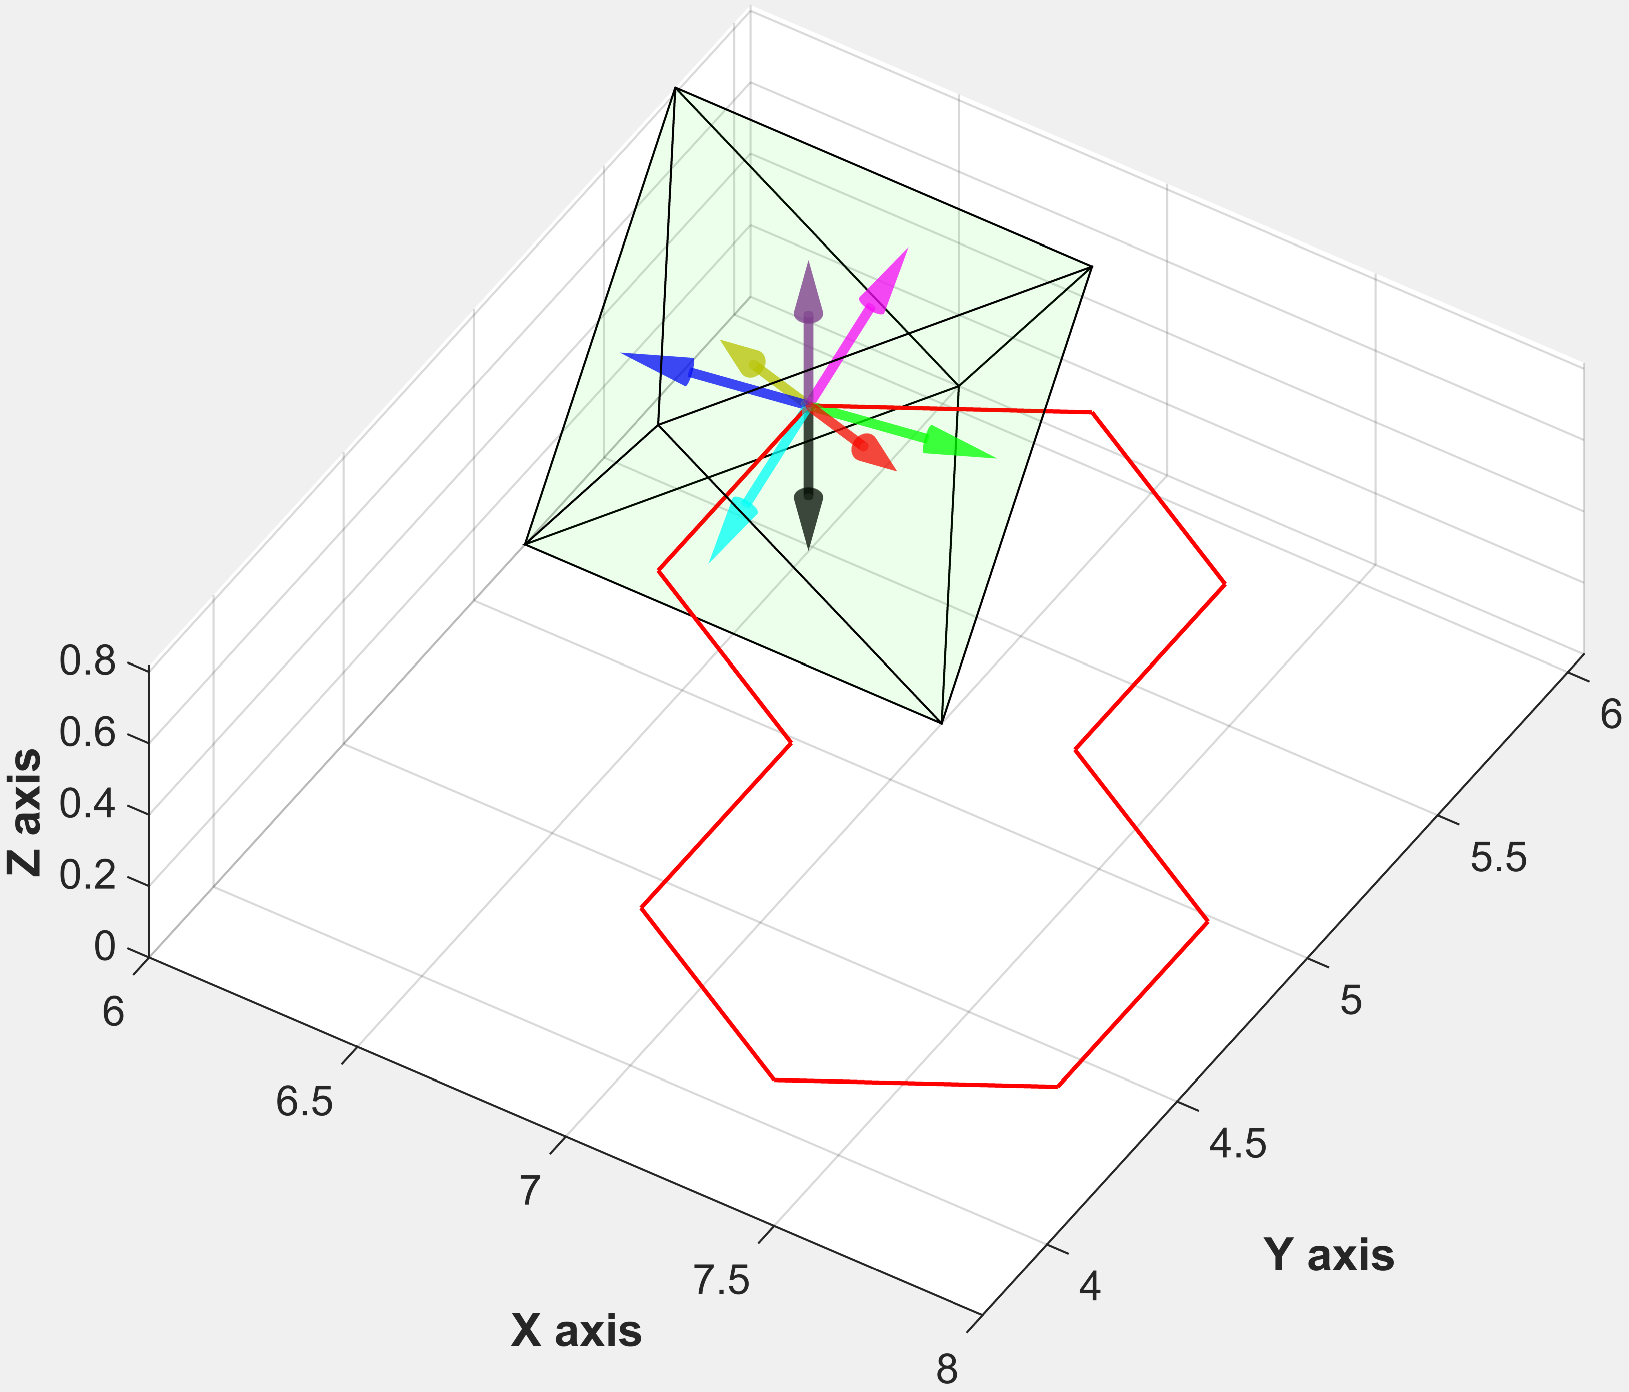
\includegraphics[width=0.5\textwidth]{image/octoPath2.pdf}
	\label{fig:Octa1Case1}
	}
\caption{Blah Blah Octa}
\end{figure}
\end{center}
%%
%%
%%
%%==================================================================================
%%
%%==================================================================================
%%
%%
%%
\clearpage
\newpage
\noindent\uline{\textbf{Icosahedron solid}}:
Writing about cube solid properties\\
This is the rolling path of icosahedron type \ref{fig:icosaPaths}.
\begin{center}
\begin{figure}[h]
\subfigure[The first shortest path of Icosahedron path rolling]{
	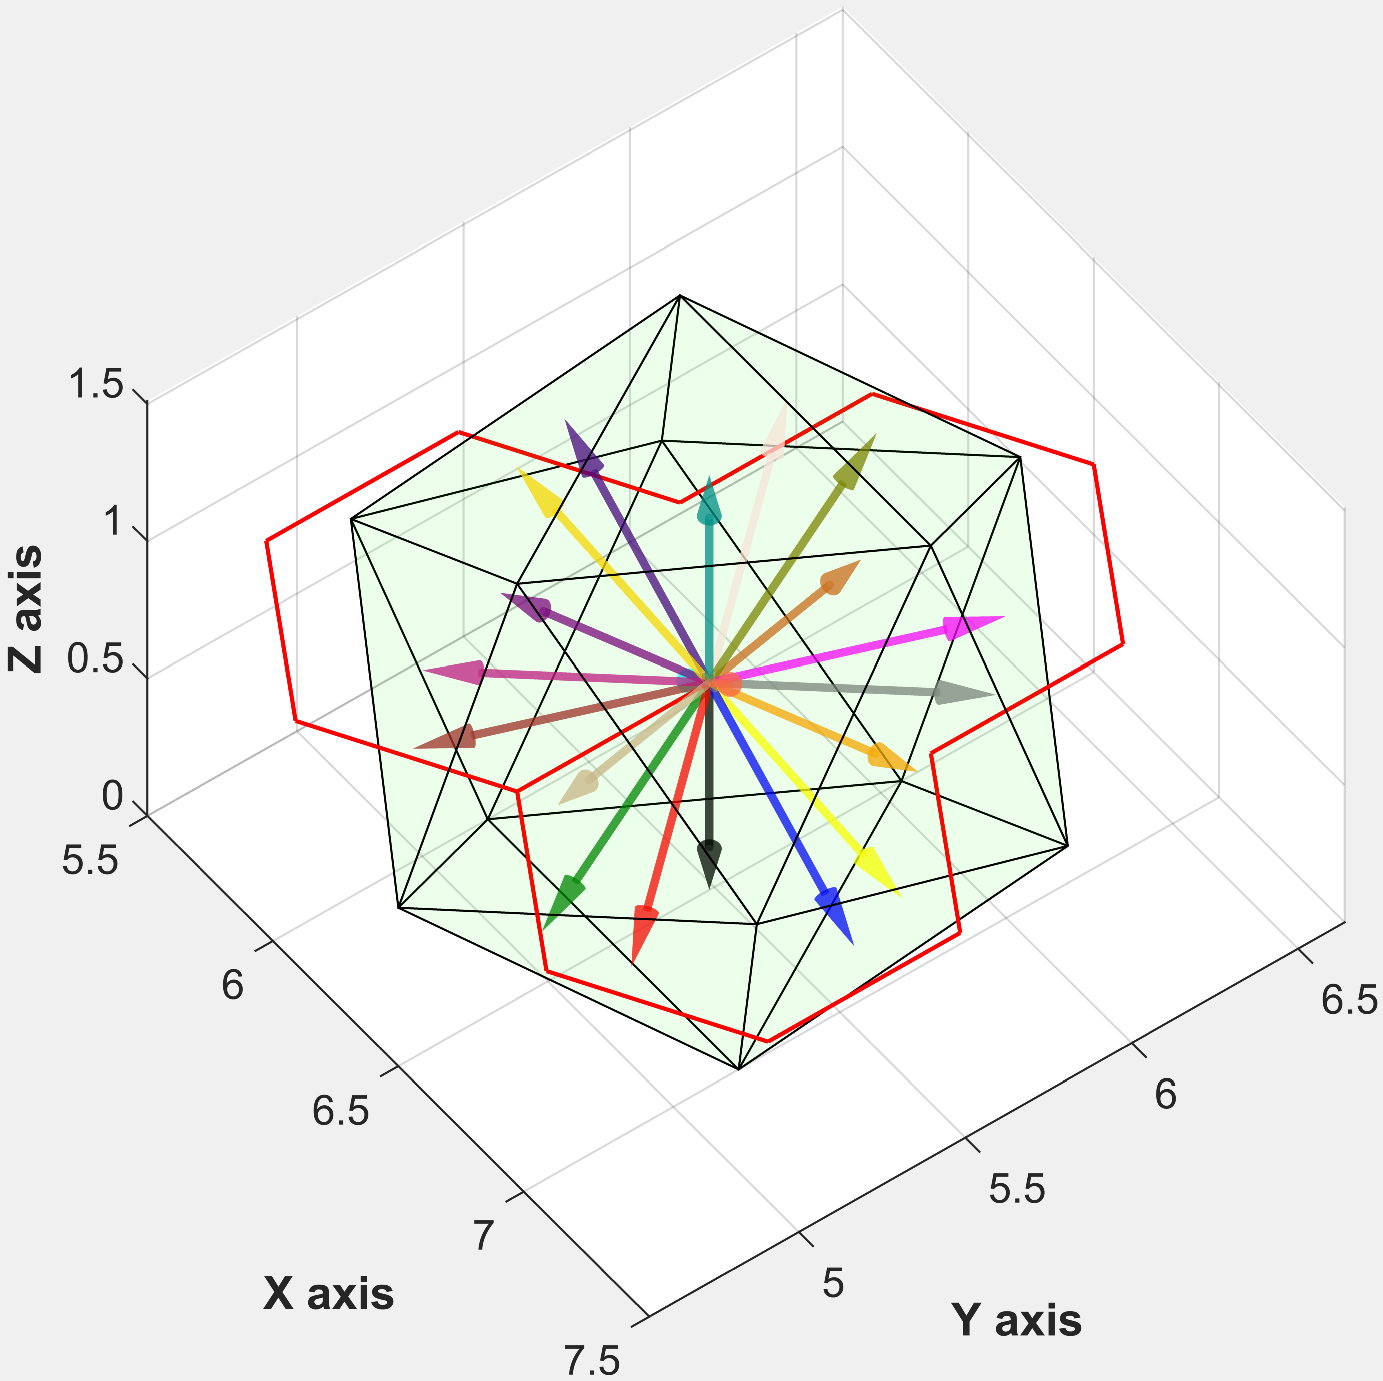
\includegraphics[width=0.5\textwidth]{image/icosaPath.pdf}
	\label{fig:Octa1Case1}
	}
\hfill
\subfigure[The top view of path planning for Icosahedron]{
	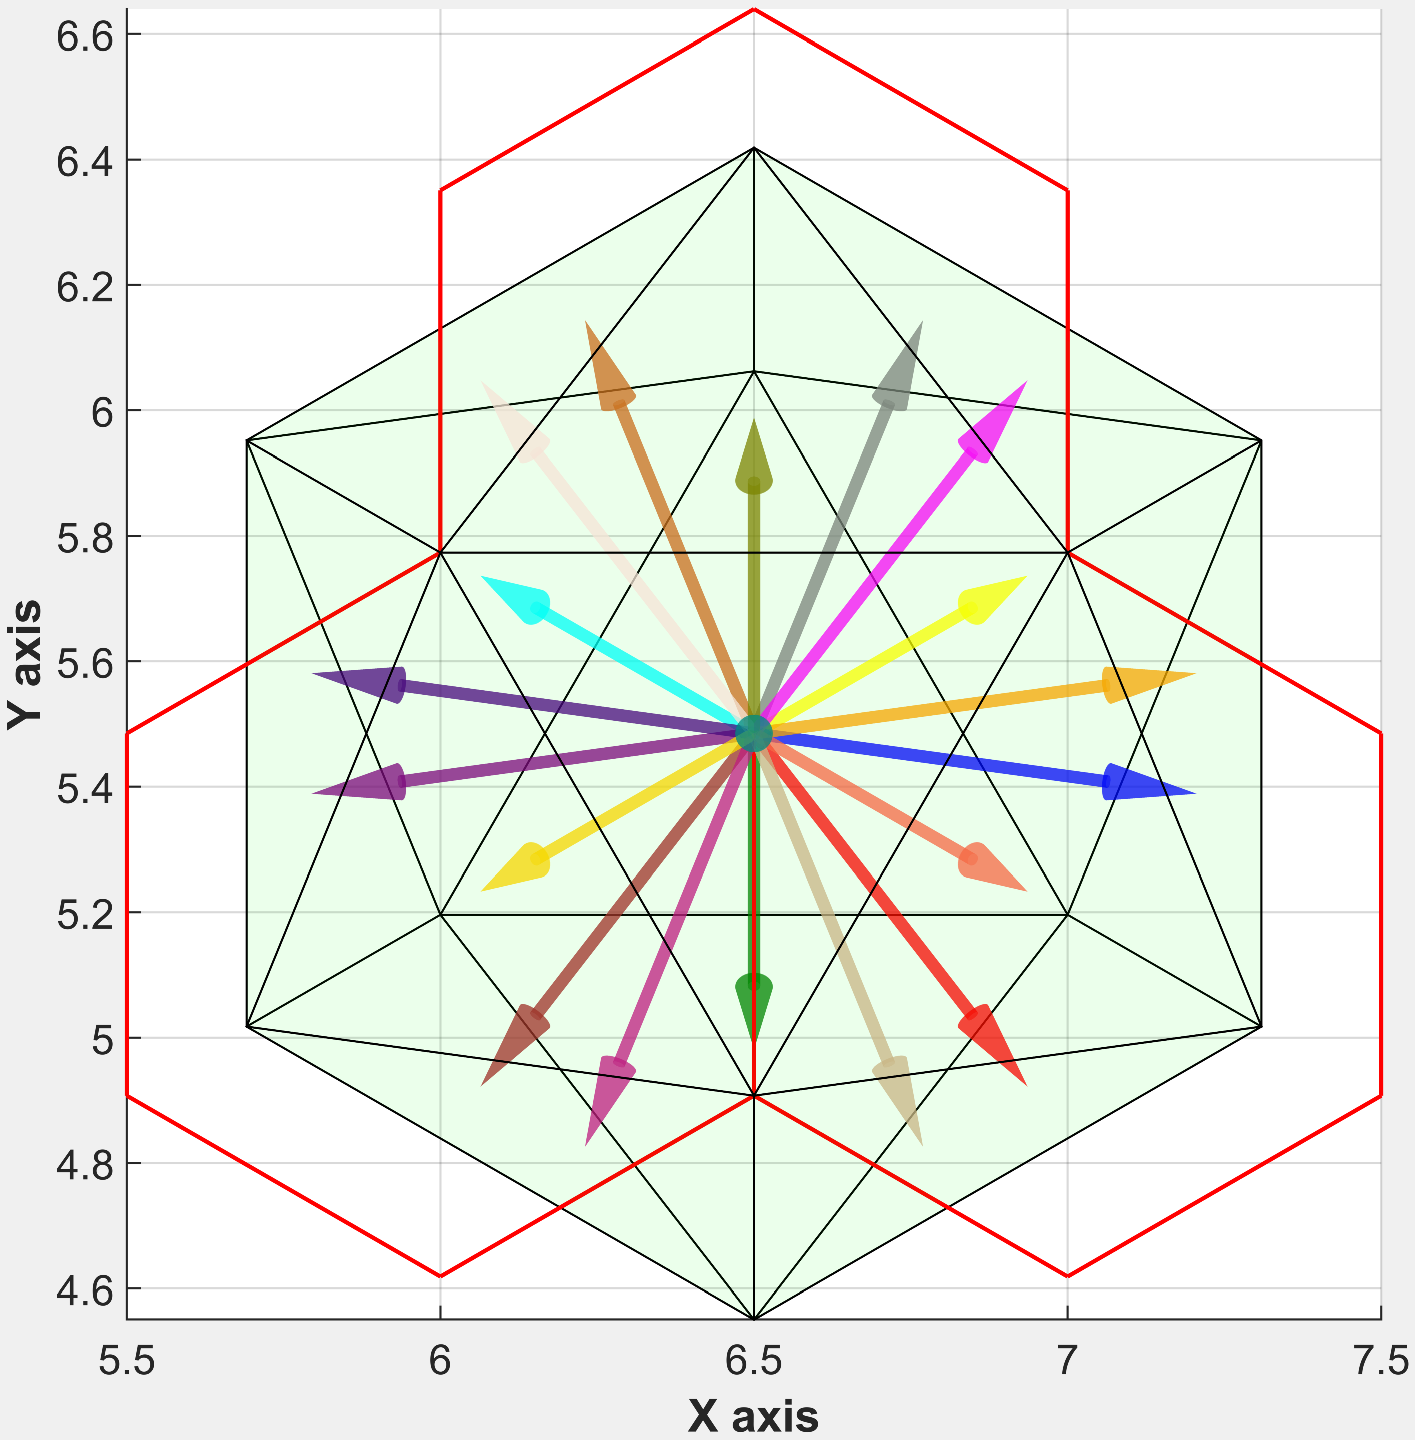
\includegraphics[width=0.5\textwidth]{image/icosaPathTopView.pdf}
	\label{fig:Octa1Case1}
	}
\caption{Blah Blah Octa}
\label{fig:icosaPaths}
\end{figure}
\end{center}
%
\clearpage
\newpage
\noindent\uline{\textbf{Dodecahedron}}:

%\noindent\uline{Result}: 
%\begin{figure}[h]
%\centering
%	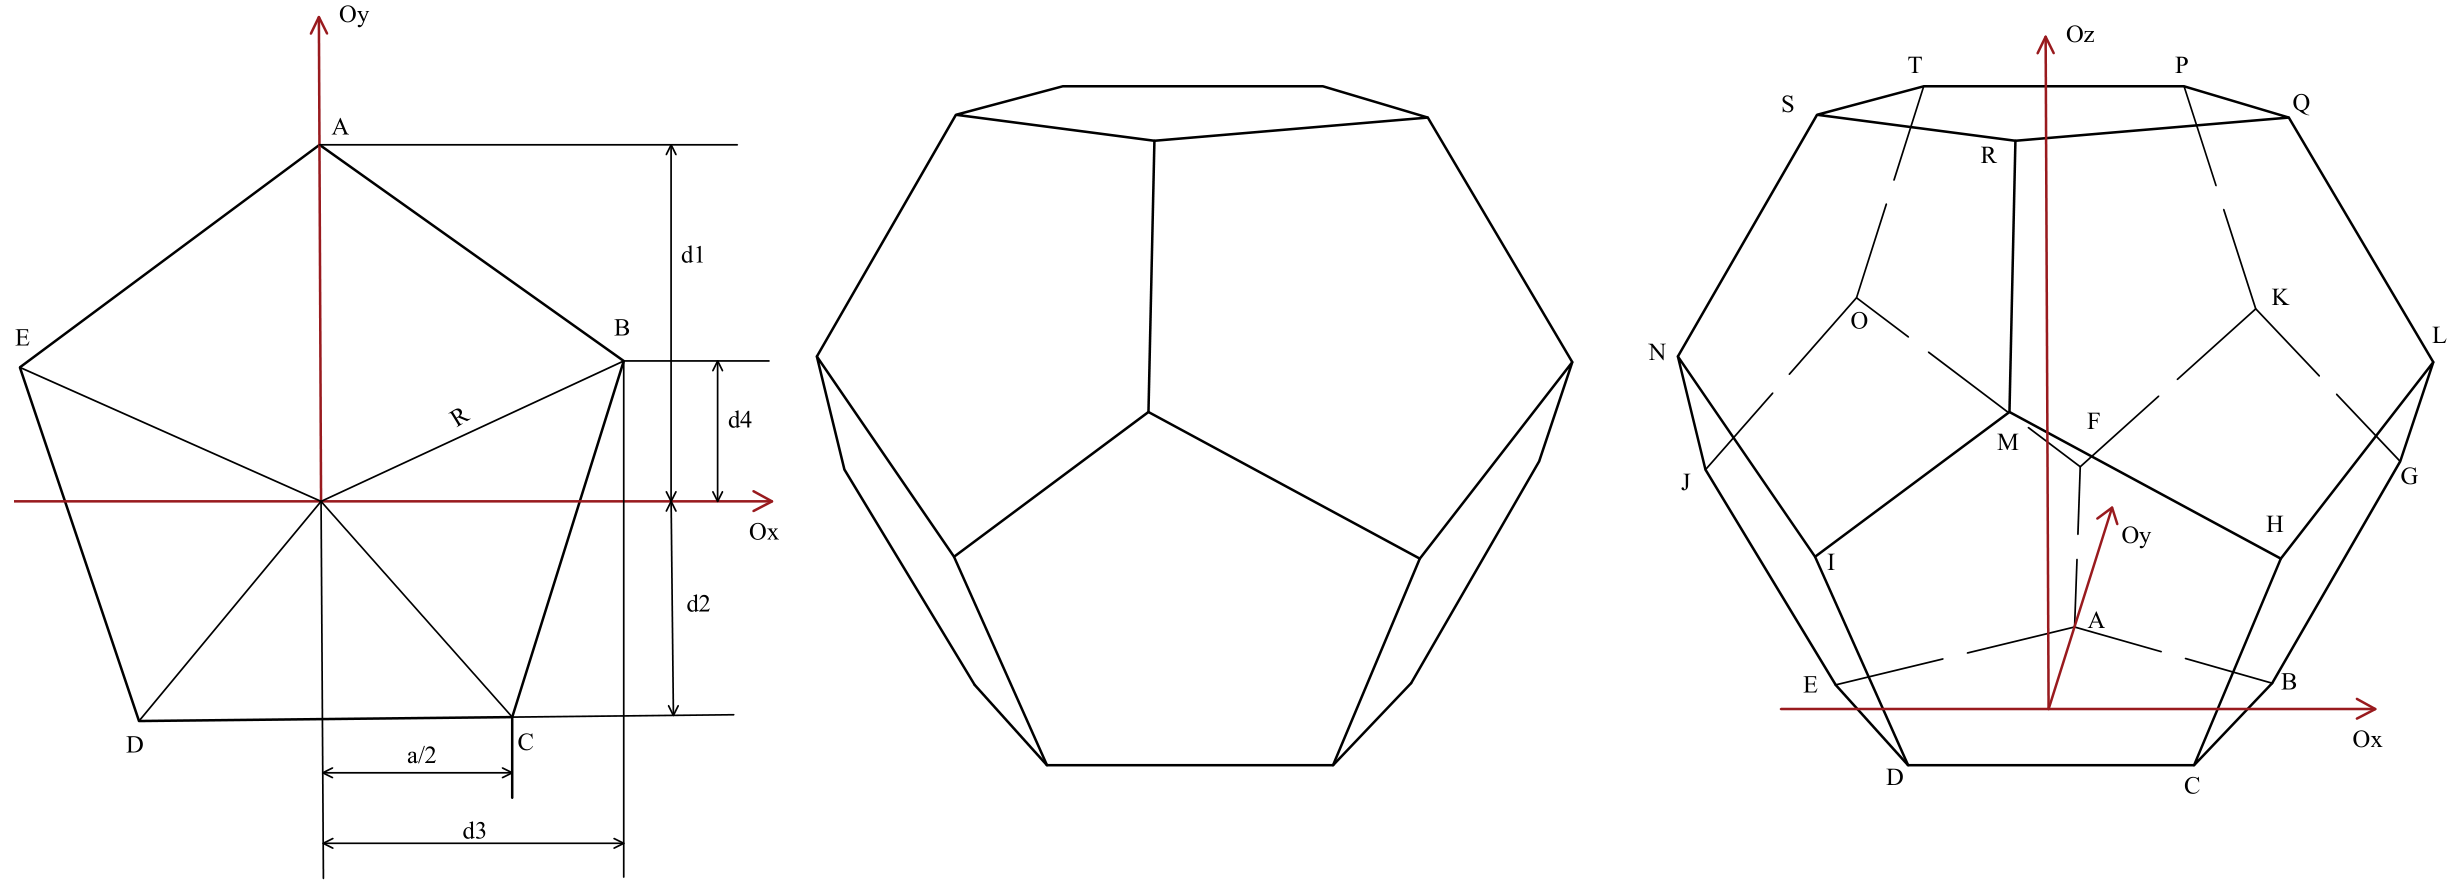
\includegraphics[width=1\textwidth]{image/dodecahedron1.png}
%	\caption{Shortest path of cube rolling}
%	\label{fig:dodecahedron1}
%\end{figure}

\noindent\uline{Properties}: 
An dodecahedron has 12 faces and 20 vertices of which generates a pentagon as shown in Figure \ref{fig:dodecahedron2}.
It will be assumed that the coordinates $Oxyz$ lie on $ABCDE$ surface within $Oy$ through $A$ and $Oz$ perpendicular to $ABCDE$.
The 30 edges have the same length as $a$. It should be determined all the vertices' coordinates in the three dimensional system.
The Figure \ref{fig:dodecahedron2} indicates the lengths of each vertices from $d_1$ to $d_4$ and the angles $\alpha_1$ to $\alpha_4$ which correspond to the five sides of a pentagon.

\begin{figure}[h]
\centering
	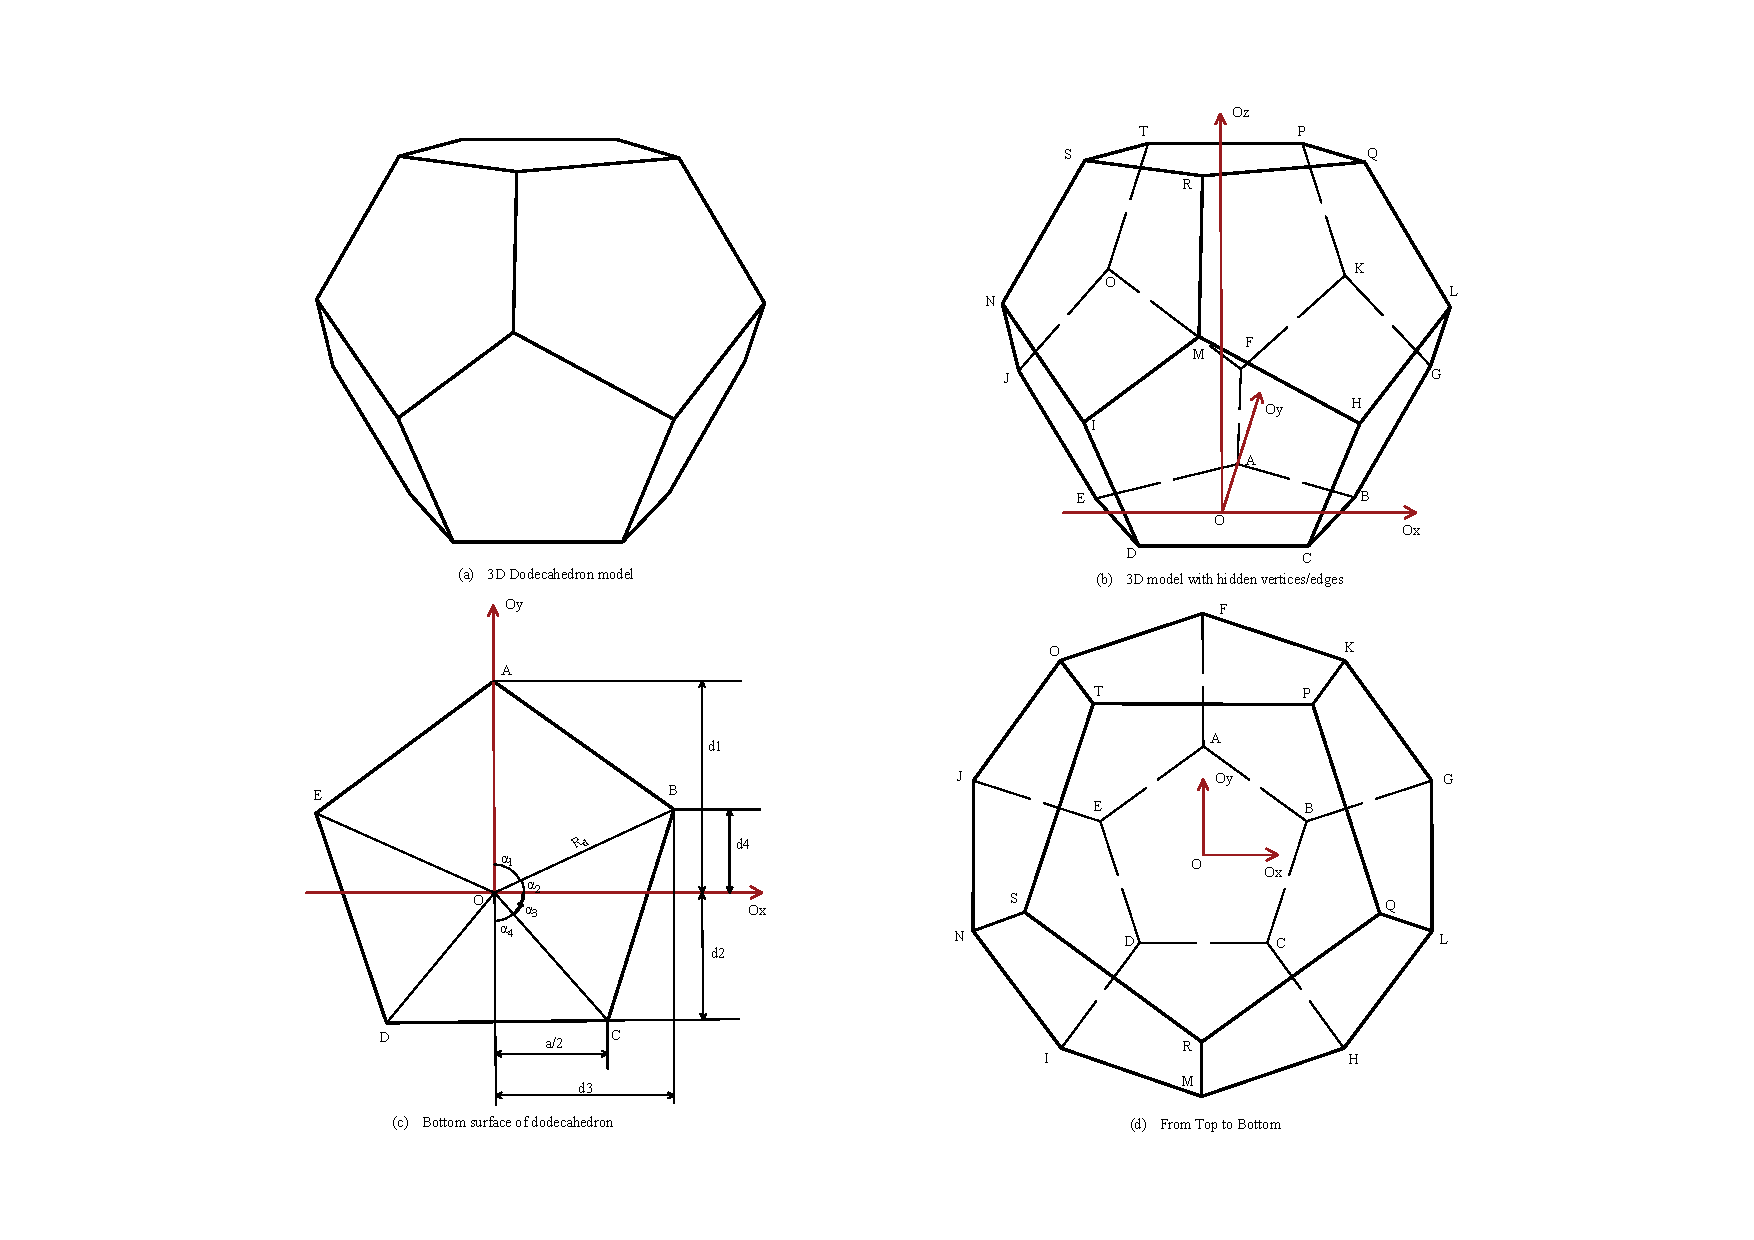
\includegraphics[width=1\textwidth]{image/dodecahedron3.pdf}
	\caption{Dodecahedron's vertices.}
	\label{fig:dodecahedron2}
\end{figure}

The path planning will implement on a surface but it will be considered in $3D$ spaces. Then, each of vertices will be determined on $3D$ coordinates such as the vertices $A$ has coordinate with $[A_x A_y A_z]$. Based on the properties of pentagon, the angle $\alpha_1=\frac{2\pi}{5}$ and $\alpha_4=\frac{\pi}{5}$. Because the angle between $Ox$ and $Oy$ is $\frac{\pi}{2}$, the sum of $\alpha_1$ and $\alpha_2$ is $\alpha_1 + \alpha_2 = \frac{\pi}{2}$. Then the other two angles $\alpha_2$ and $\alpha_3$ can be determined by $\alpha_2 = \frac{\pi}{2}-\alpha_1 = \frac{\pi}{2}-\frac{2\pi}{5} = \frac{\pi}{10}$ and $\alpha_3 = \alpha_1-\alpha_2 = \frac{2\pi}{5}-\frac{pi}{10} = \frac{3\pi}{10}$.\\

From the Figure \ref{fig:dodecahedron2}(c), these labelled dimensions can be calculated as $d_1 = R_d = \frac{a}{2\sin{\alpha_4}}$ with $R_d$ is the circumradius of dodecahedron, $d_2 = d_1\cos{\alpha_4}$, $d_3 = d_1\cos{\alpha_2}$, and $d_4 = d_1\sin{\alpha_2}$. Referencing to the properties of a dodecahedron with length $a$, the radius of an inscribed sphere is $r_i = \frac{a}{20}\sqrt{10(25+11\sqrt{5})}$ and the circumscribed sphere radius is $r = a\frac{\sqrt{3}}{2}\frac{1+\sqrt{5}}{2}$.\\

There are total $20$ vertices of a dodecahedron. This article focuses on the rolling contact to $2D$ surface, the bottom surface of the dodecahedron integrated to the $Oxy$ which contact to the $2D$ surface. This condition express the $Oz$ dimension of the vertices $ABCDE$ equal to $0$ or $A_z = B_z = C_z = D_z = E_z = 0$. Then $P_z = Q_z = R_z = S_z = T_z = 2.r_i = \frac{a}{10}\sqrt{10(25+11\sqrt{5})}$.\\

It can be seen that the distance $|AF|$ is $a$ and the distance $|BF|$ is $2d_3$. Using the distance properties and squaring the results give:
\begin{equation} 
\label{dodeca:eq1}
\begin{split}
AF^2 & = a^2 = (A_x-F_x)^2 + (A_y-F_y)^2 + (A_z-F_z)^2 \\
BF^2 & = (2d_3)^2 = (B_x-F_x)^2 + (B_y-F_y)^2 + (B_z-F_z)^2
\end{split}
\end{equation}

Figure \ref{fig:dodecahedron2}(d) shows that $A_x = F_x = 0$, $A_y = d_1$, $B_y = d_4$, $B_x = d_3$, $A_z = B_z$. Define $d_5=A_z-F_z$, the relations of these equations are:
\begin{equation} 
\label{dodeca:eq2}
\begin{split}
a^2 & = (F_y-d_1)^2 + d_5^2\\
(2d_3)^2 & = (F_y-d_4)^2 + d_5^2 + d_3^2
\end{split}
\end{equation}

Solving $F_y$ and $d_5$ gives:
\begin{equation} 
\label{dodeca:eq3}
\begin{split}
F_y & = \frac{a^2-(2d_3)^2-(d_1^2-d_3^2-d_4^2)}{2(d_4-d_1)} \\
d_5 & = \frac{1}{\sqrt{2}}\sqrt{a^2+(2d_3)^2-(F_y-d_1)^2-(F_y-d_4)^2-d_3^2}
\end{split}
\end{equation}

From these equations \ref{dodeca:eq1},\ref{dodeca:eq2},\ref{dodeca:eq3}, all the vertices will be founded in the three-dimensional space. Path planning based on rolling is the motion of all these vertices through edges' contact.


%%
%%
%%
%%==================================================================================
%
%\begin{figure}[h]
%\centering
%	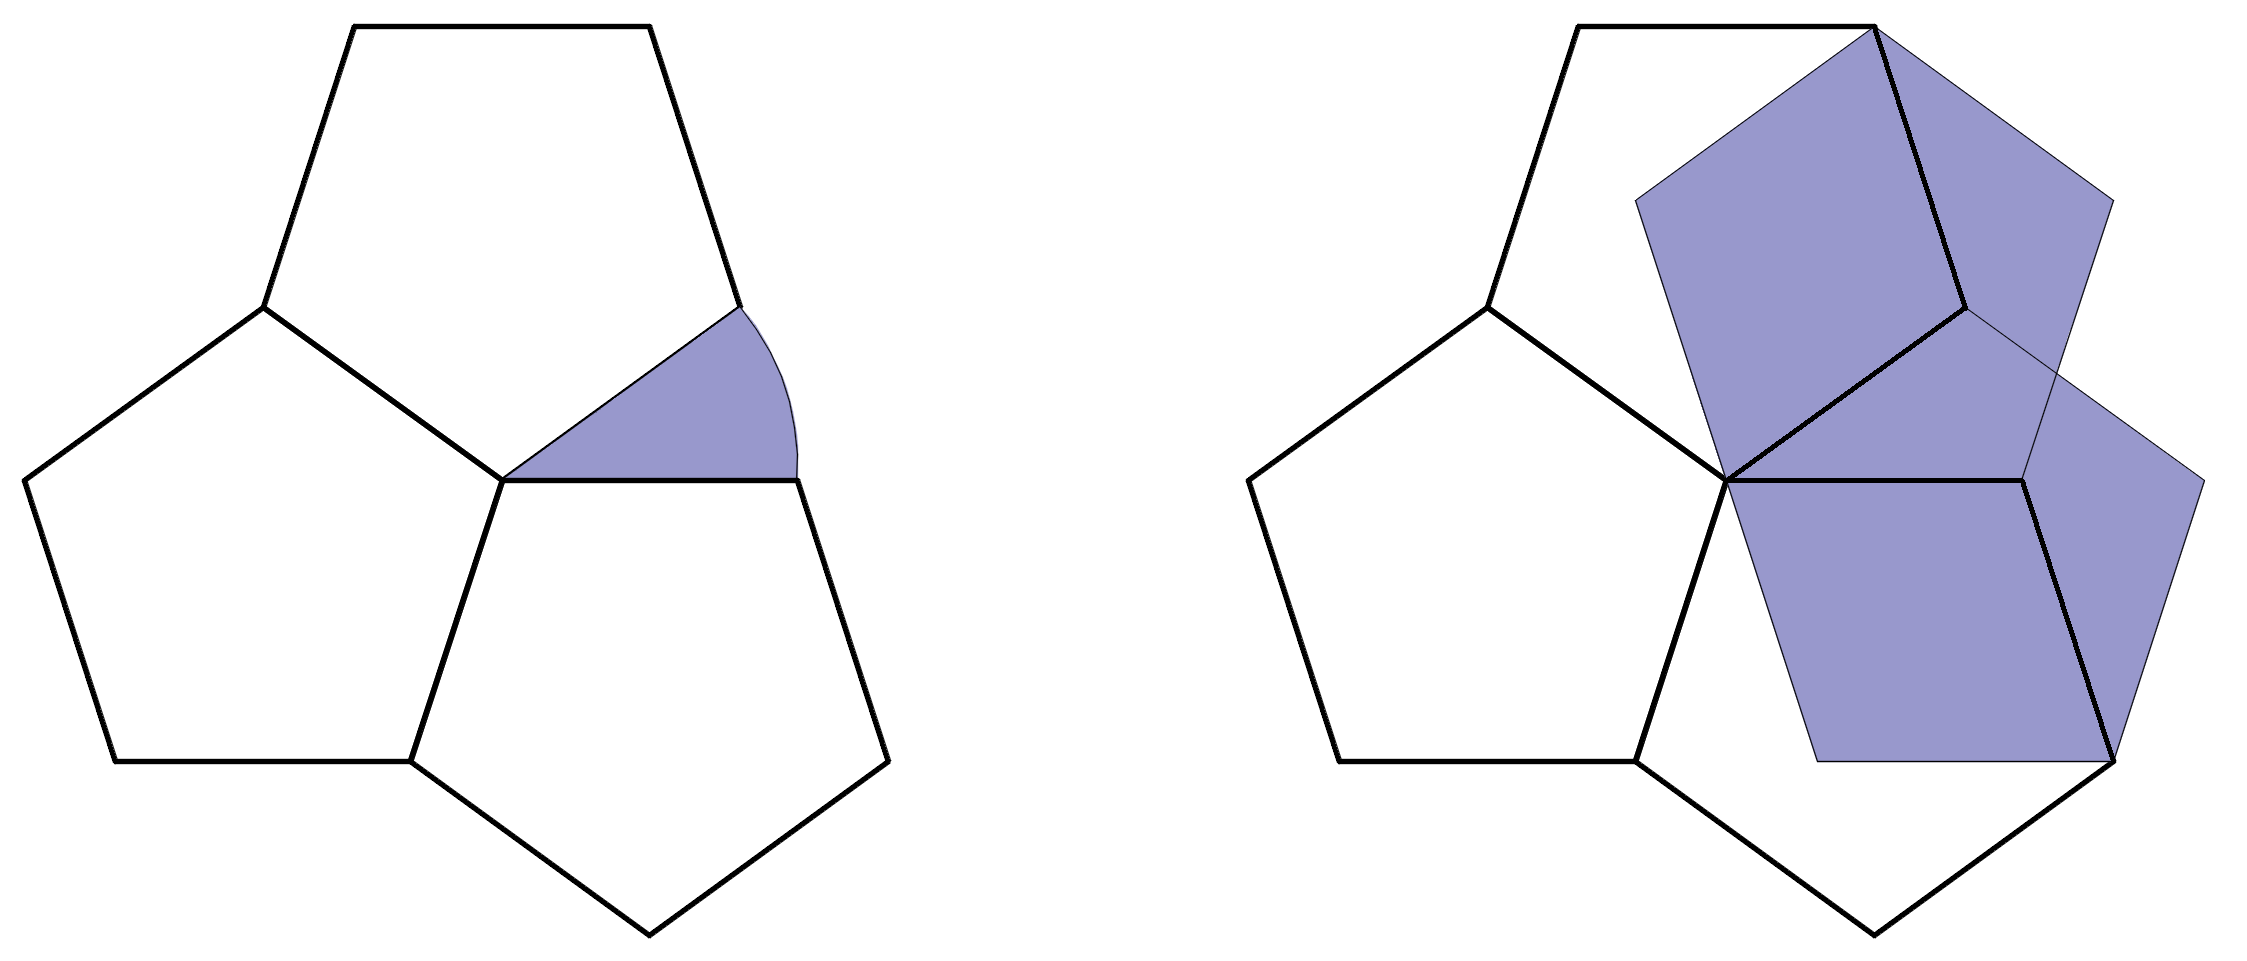
\includegraphics[width=1\textwidth]{image/dodecaOverlap.png}
%	\caption{Pentagons connect around a point with a gap and overlap}
%	\label{fig:dodecaOverlap}
%\end{figure}
%%==================================================================================
%%
%%
%%
\newpage
\noindent\uline{\textbf{Experiments}}:
Writing about cube solid properties\\

\noindent\uline{\textbf{Discussion}}: 
\textcolor{blue}{Q2 \& Q3\\
- Q2: What are the new things you learned after you did whatever you did?\\
- Q3: What exactly did you do?}\\

\begin{itemize}
\color{red}
\item \textbf{Discussion}
\item \textit{What your results mean}
\item \textit{Why it makes a difference}
\item \textbf{Conclusion}
\item \textit{Broader implications}
\item \textit{Areas for further study}
\end{itemize}





